 \section{Analysing the pre-existing PIPE codebase}
The PIPE codebase was found to suffer from poor coding practices (see~\cref{lst:identical}). So numerous were these instances it was necessary to use automated analysis to track down them all. Indeed the QAPlug plug-in for IntelliJ found a total of \num{12904} code quality issues as shown in \cref{fig:qaplug}.

A structural analysis of PIPE 4 was performed by the Stan4J standalone tool. It reports cyclic dependencies as tangles and considers a tangle to be `A subgraph with at least two nodes, where each node is reachable from each other. Every cycle lies in a tangle and every tangle consists of just cycles'~\cite{stan_whitepaper}. It reports PIPE 4 as 29.17\% tangled which is shown diagrammatically in~\cref{fig:tangle}.

In modern day programming it is considered good practice for classes and methods to be short, composed of auxiliary methods and to have a single purpose~\cite{so_can_a_function_be_too_short}. Unfortunately PIPE 4 has many large classes, some with over \num{3000} lines of code. 

\begin{figure}[H]
\begin{center}
\begin{lstlisting}[frame=single]
private String compareTransitions(...) {
  if((!compareID || source[i].getId().equals(comparison[j].getId())) &&
    (!compareName || source[i].getName().equals(comparison[j].getName())) &&
    (!compareMarking || source[i].getCurrentMarkingView().get(0).getCurrentMarking()
      == comparison[j].getCurrentMarkingView().get(0)
      .getCurrentMarking()) &&
    (!compareCapacity || source[i].getCapacity() == comparison[j].getCapacity()))
    {
      s = "Identical";
    }
}
\end{lstlisting}
  
\caption{A snippet of the code used to determine equality and similarities between
            Petri nets in PIPE 4. Similar code appears 3 times within the same class.}
\label{lst:identical}
\end{center}
\end{figure}

% \mediumlinespacing
\begin{figure}[tbp]
\begin{framed}
\begin{itemize}
    \item \textcolor{red}{\textbf{Efficiency: 225}}
    \begin{itemize}
        \item \textit{`Performance -  Method concatenates strings using + in a loop count: 44'} --- In each iteration, the String is converted to a StringBuffer/StringBuilder, appended to, and converted back to a String. This can lead to a cost quadratic in the number of iterations, as the growing string is recopied in each iteration. Better performance can be obtained by using a StringBuffer (or StringBuilder in Java 1.5) explicitly.
        \item \textit{`Avoid Array Loops count: 3 - System.arraycopy is more efficient'} --- Instead of copying data between two arrays, use System.arrayCopy method.
    \end{itemize}

    \item \textcolor{red}{\textbf{Maintainability: 1803}}
    \begin{itemize}
        \item \textit{`Avoid duplicate literals count: 160'} --- Can usually be improved by declaring the String as a constant field.
        \item \textit{`Bad practice - Comparison of string objects using == or != count: 7'} --- This code compares java.lang.String objects for reference equality using the == or != operators. Consider using the equals(Object) method instead.
        \item \textit{`God class count: 66'} --- The God class rule detects the God Class design flaw using metrics. God classes do too many things, are very big and overly complex. They should be split apart to become more object-orientated. 
    \end{itemize}
      
     \item \textcolor{red}{\textbf{Portability: 47}} 
    \begin{itemize}
        \item \textit{`Replace Vector With List count: 22'} ---
            Consider replacing Vector usages with the newer 
        java.util.ArrayList if expensive thread-safe operation is not required.
        \item \textit{`Integer Instantiation count: 19'} --- Calling new Integer() causes memory allocation. Integer.valueOf() is more memory friendly.
    \end{itemize}
    
    \item \textcolor{red}{\textbf{Reliability: 1847}}
    \begin{itemize}
        \item \textit{`Malicious code vulnerability - May expose internal representation by returning reference to mutable object count: 10'}. --- Returning a reference to a mutable object value stored in one of the object's fields exposes the internal representation of the object. Returning a new copy of the object is better approach in many situations.
        \item \textit{`Magic Number count: 1385'} --- Checks for magic numbers.
    \end{itemize}

    \item \textcolor{red}{\textbf{Usability: 8982}}
    \begin{itemize}
        \item \textit{`Dodgy - write to static field from instance method count: 49'} --- This instance method writes to a static field. This is tricky to get correct if multiple instances are being manipulated, and generally bad practice. 
        \item \textit{`System Println count: 412'} --- System.(out|err).print is used, consider using a logger.
        \item \textit{`Code Too Long count: 15'} --- Method is too long.

    \end{itemize}
\end{itemize} 
\end{framed}
\caption{Examples of interesting code quality issues highlighted by the QAPlug plug-in for IntelliJ for the pre-existing PIPE 4 codebase.}
\label{fig:qaplug}
\end{figure}
% \normallinespacing

\begin{figure}[tb]
\begin{center}
    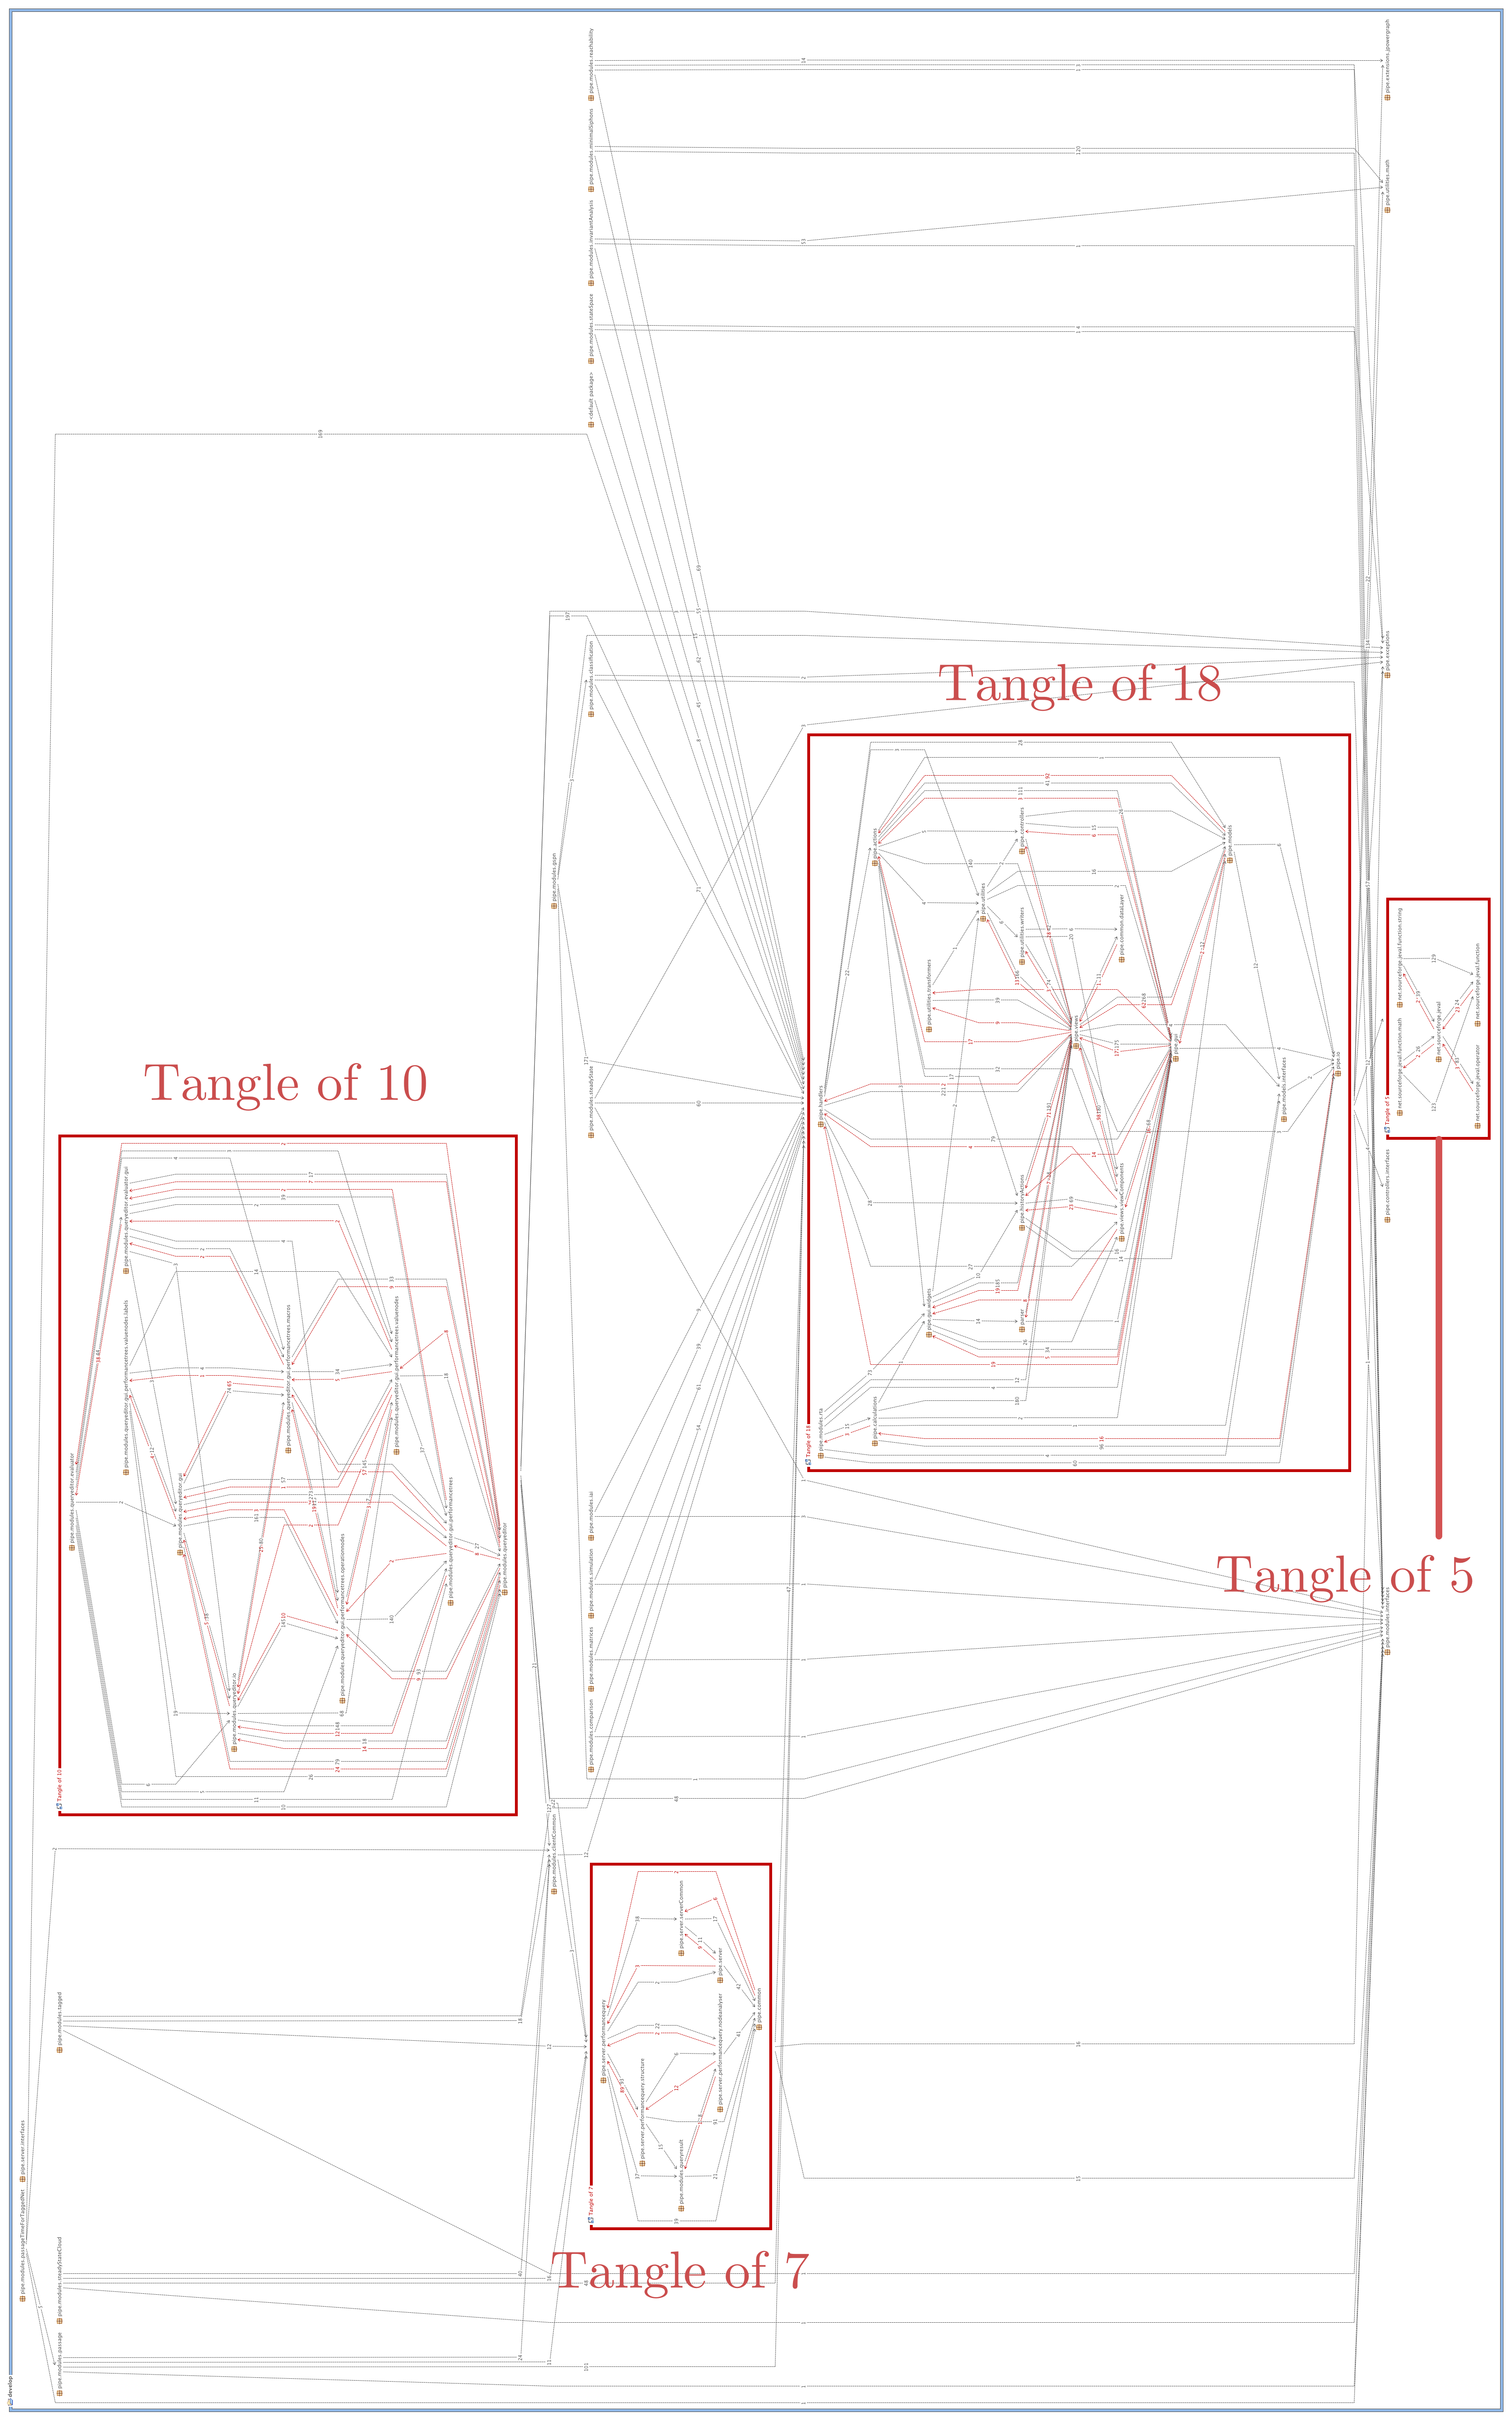
\includegraphics[width=0.7\textwidth]{analysis/tangle_annotated.png} 
    \caption{Stan4J tangle graph of the entire PIPE 4 codebase. It has 4 distinct tangles which are of sizes 18, 10, 7 and 5.}
    \label{fig:tangle}
\end{center}
\end{figure}